\section{سرعت بخشی}
\begin{frame}[standout]
\begin{latin}
	HOSVD for Dimensionality Reduction
	\end{latin}
\end{frame}
\begin{frame}
{مقدمه}
\small{
فرض کنید 
$M_1\in \mathbb{R}^{m_1\times n}$
و
$M_2\in \mathbb{R}^{m_2\times n}$
که 
$m_1<m_2$
است و 
$M_2=[M_1,~~0]$.

هرگاه تجزیه $SVD$ آن‌ها به صورت زیر باشد:
\begin{align*}
M_1=&U_1\Sigma_1V_1^T\\
M2=&U_1\Sigma_1V_1^T
\end{align*}
در این صورت ماتریس متعامد $U_1$ معادل با $U_2$ است.

\pause
\textbf{نتیجه:}
فرض کنید 
$M_1=[v_1,\cdots,v_n]$
و
$M_2=[v_1,v_2,\cdots,0,\cdots,0,v_n]$،
در این صورت پایه‌هی معادل دارن.
}
\end{frame}
\begin{frame}{معادل بودن تانسوری هسته در $HOSVD$}
فرض کنید 
$T\in \mathbb{R}^{I_1\times\cdots I_N}$
و
$G\in \mathbb{R}^{I_1\times\cdots\times(kI_n)\times\cdots I_N}$
باشد.
با در نظر گرفتن ماتریس
\[
M=\begin{pmatrix}
I\\0
\end{pmatrix},\qquad M\in\mathbb{R}^{I_n\times (kI_n)}
\]
تانسور  $T$ و $G$ در رابطه زیر صدق می‌کند:
\[T=G\times_nM=G\times_n\begin{pmatrix}
I_n\\0_{kn}
\end{pmatrix},\]
\end{frame}
\begin{frame}{IHOSVD}
این روش شامل سه الگوریتم است که در اولین الگوریتم، یک الگوریتم بازگشتی می‌باشد که تابع زیر را بدست می‌آورد:
\begin{align*}
f(M_n,C_n)=
\begin{cases}
svd(M_1),& n=1\\
mix(f(M_{n-1},C_{n-1}),C_n),&n>1
\end{cases}
\end{align*}
\end{frame}
\begin{frame}{IHOSVD}
\begin{center}
	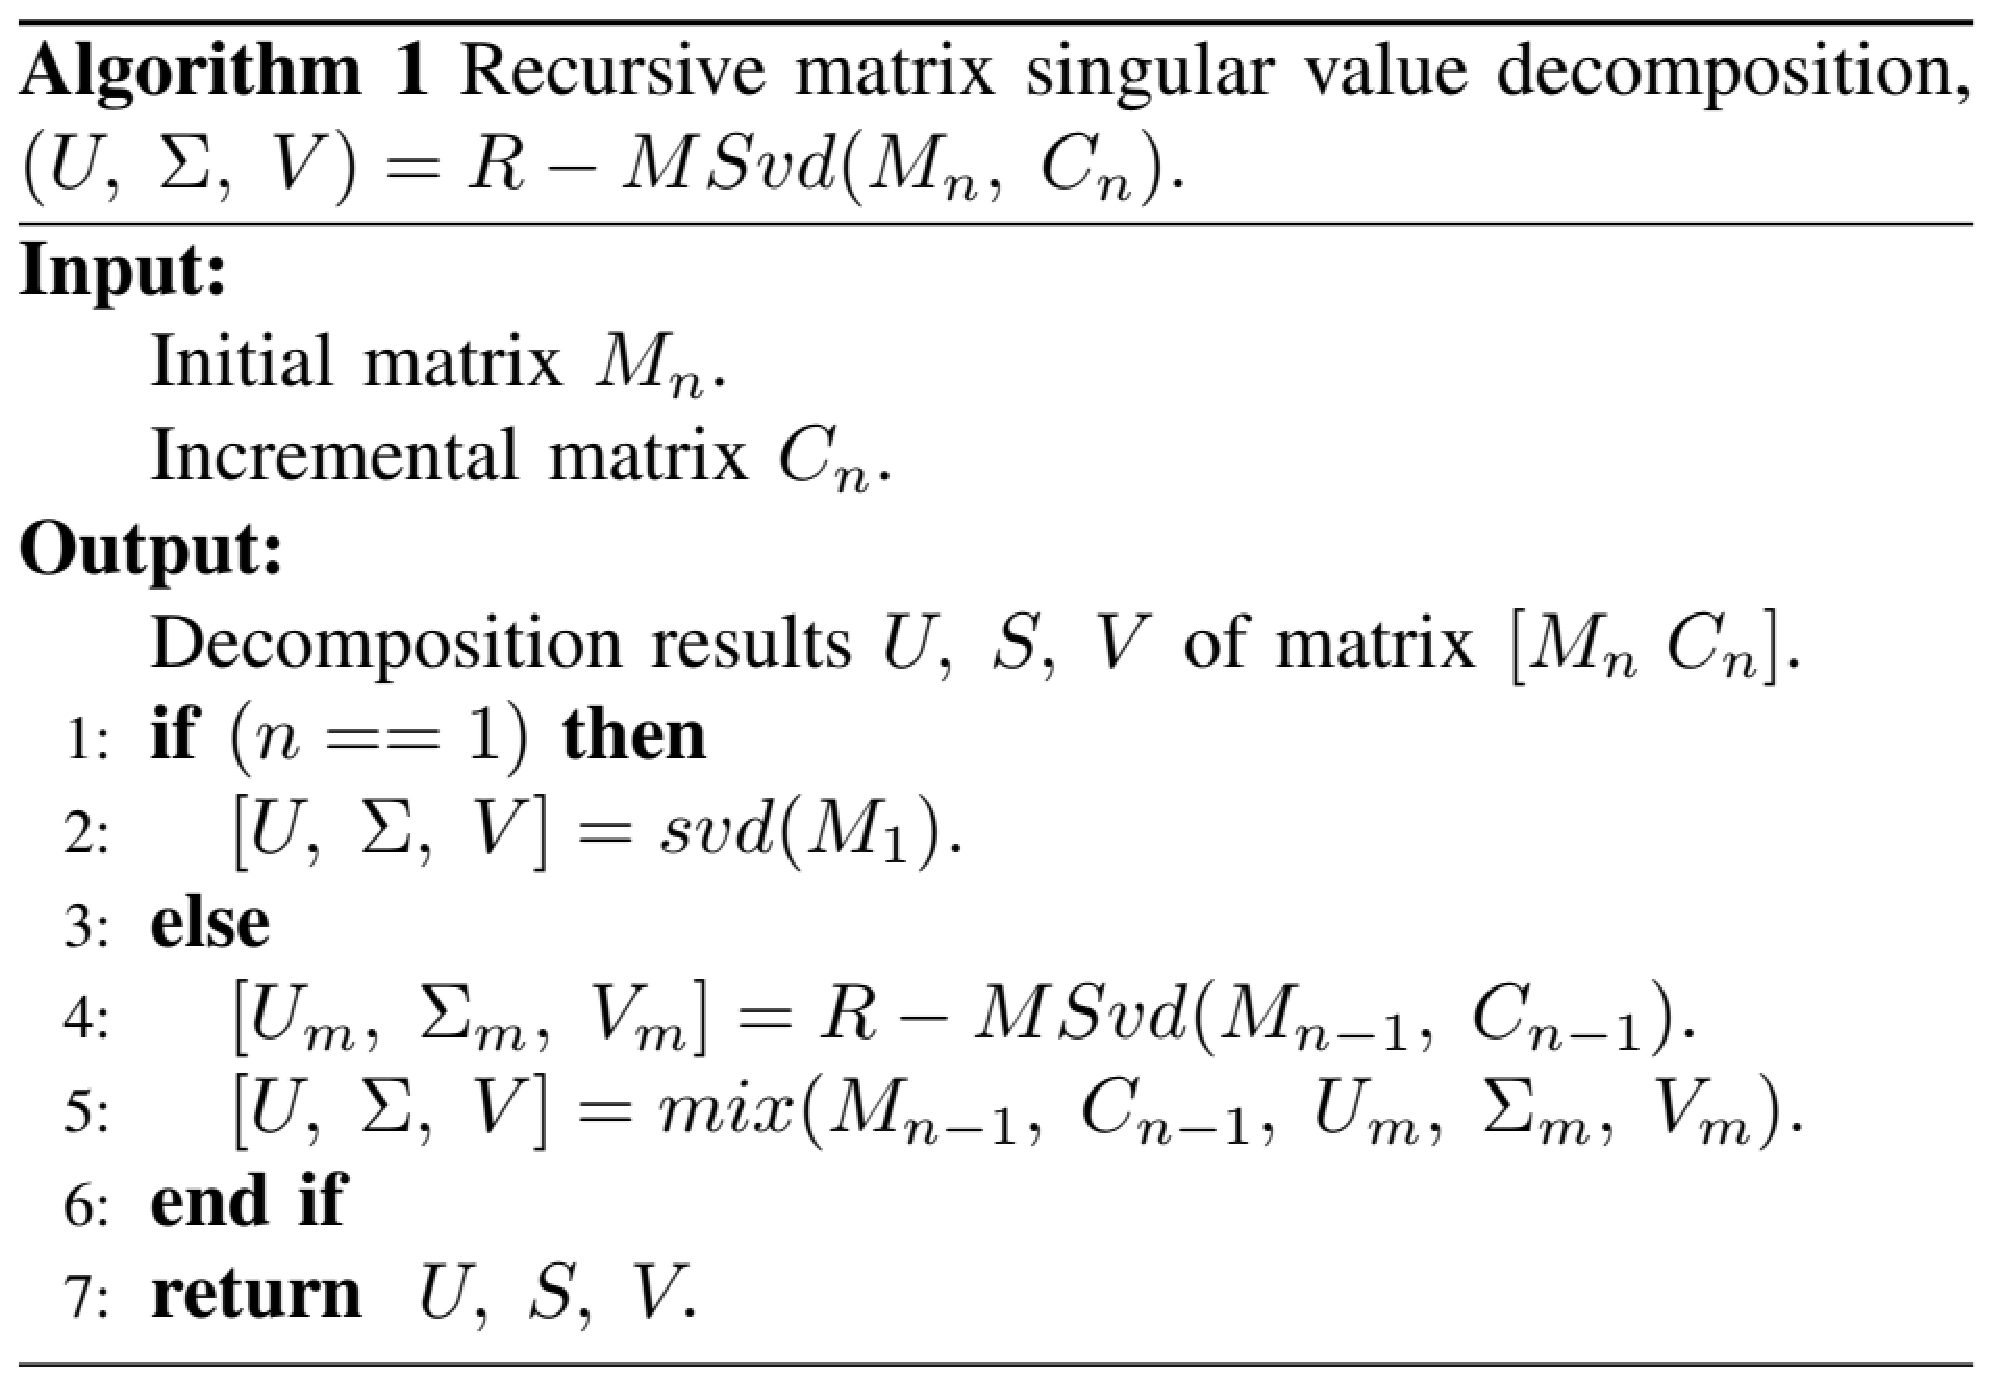
\includegraphics[width=.8\textwidth]{img/ok/AIHOSVD.pdf}
\end{center}
\end{frame}
\begin{frame}{IHOSVD}
دومین الگوریتم، $SVD$ را بروزرسانی می‌کند. از ورودی ماتریس $C_{n-1}$ را خوانده و به فضای متعامد تولید شده از $U_m$ تصویر می‌کند.
\begin{center}
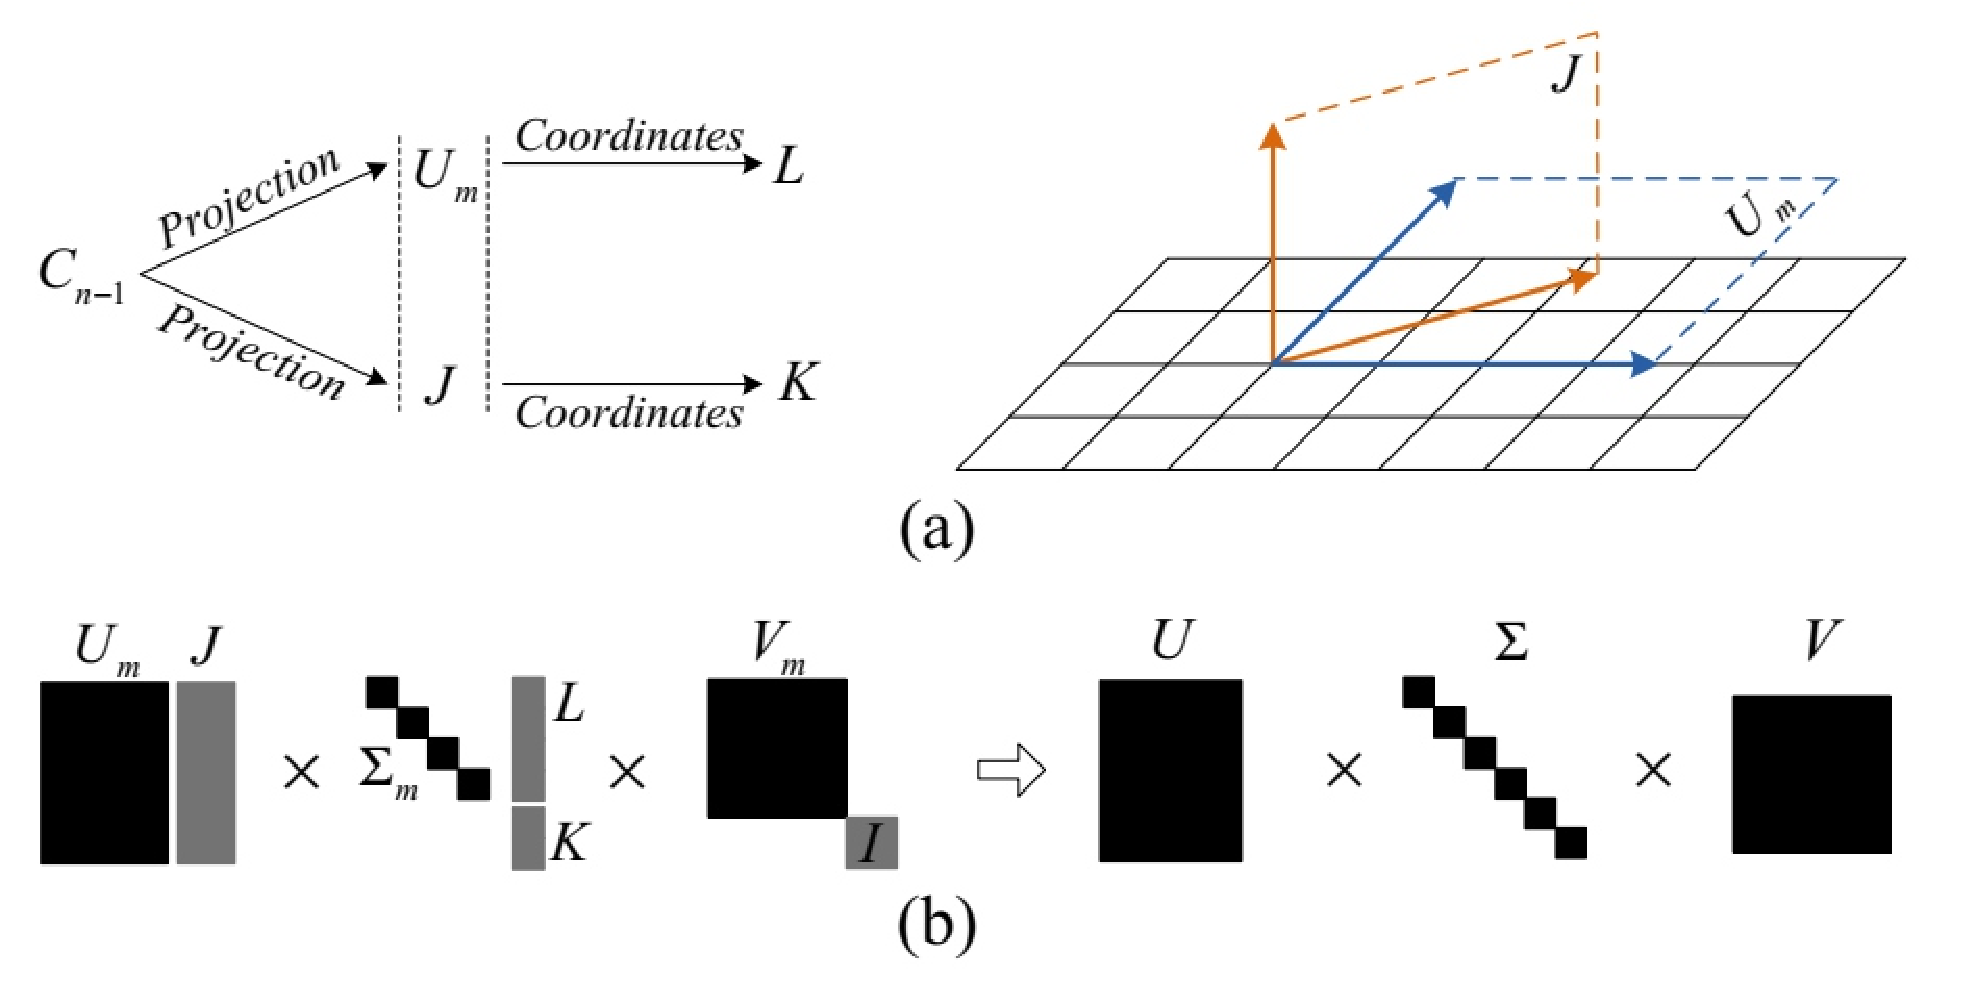
\includegraphics[width=.8\textwidth]{img/ok/fig8.pdf}
\end{center}
\end{frame}
\begin{frame}
\begin{center}
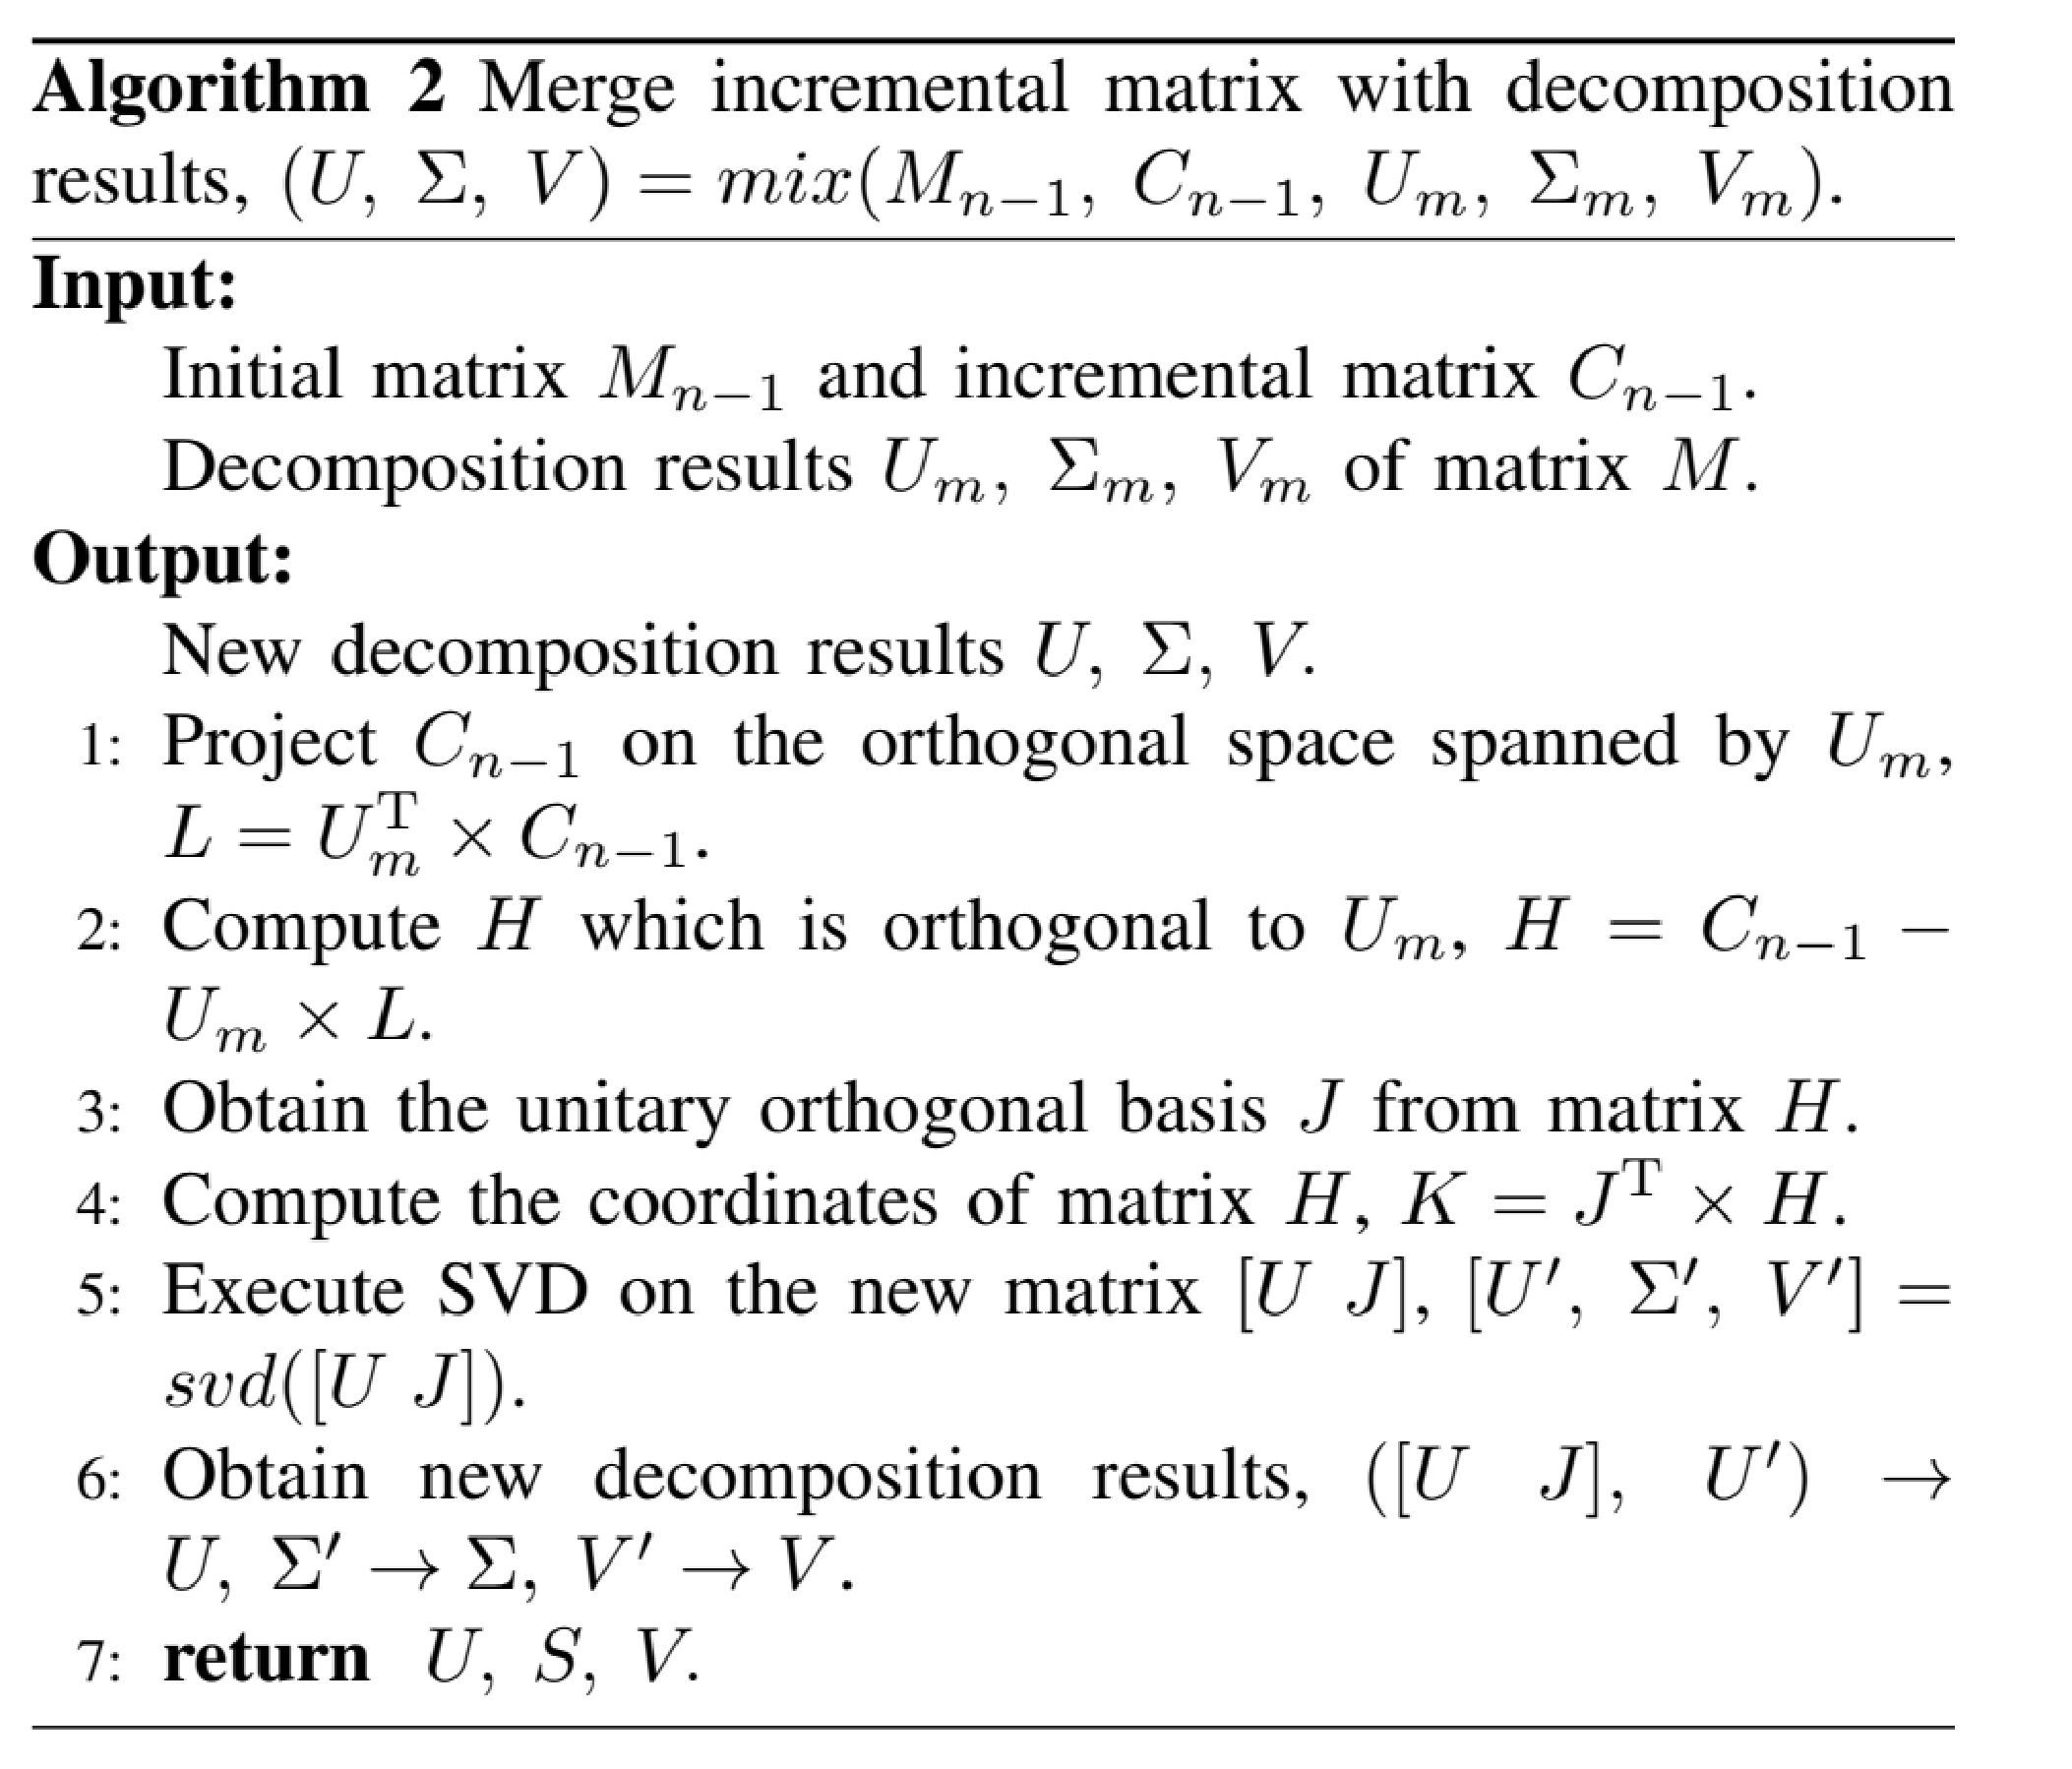
\includegraphics[width=.8\textwidth]{img/ok/AIHOSVD2.pdf}
\end{center}
\end{frame}
\begin{frame}{IHOSVD}
با استفاده از سومین الگوریتم  ما هسته تانسور را حساب خواهیم کرد.

\pause
\begin{center}
	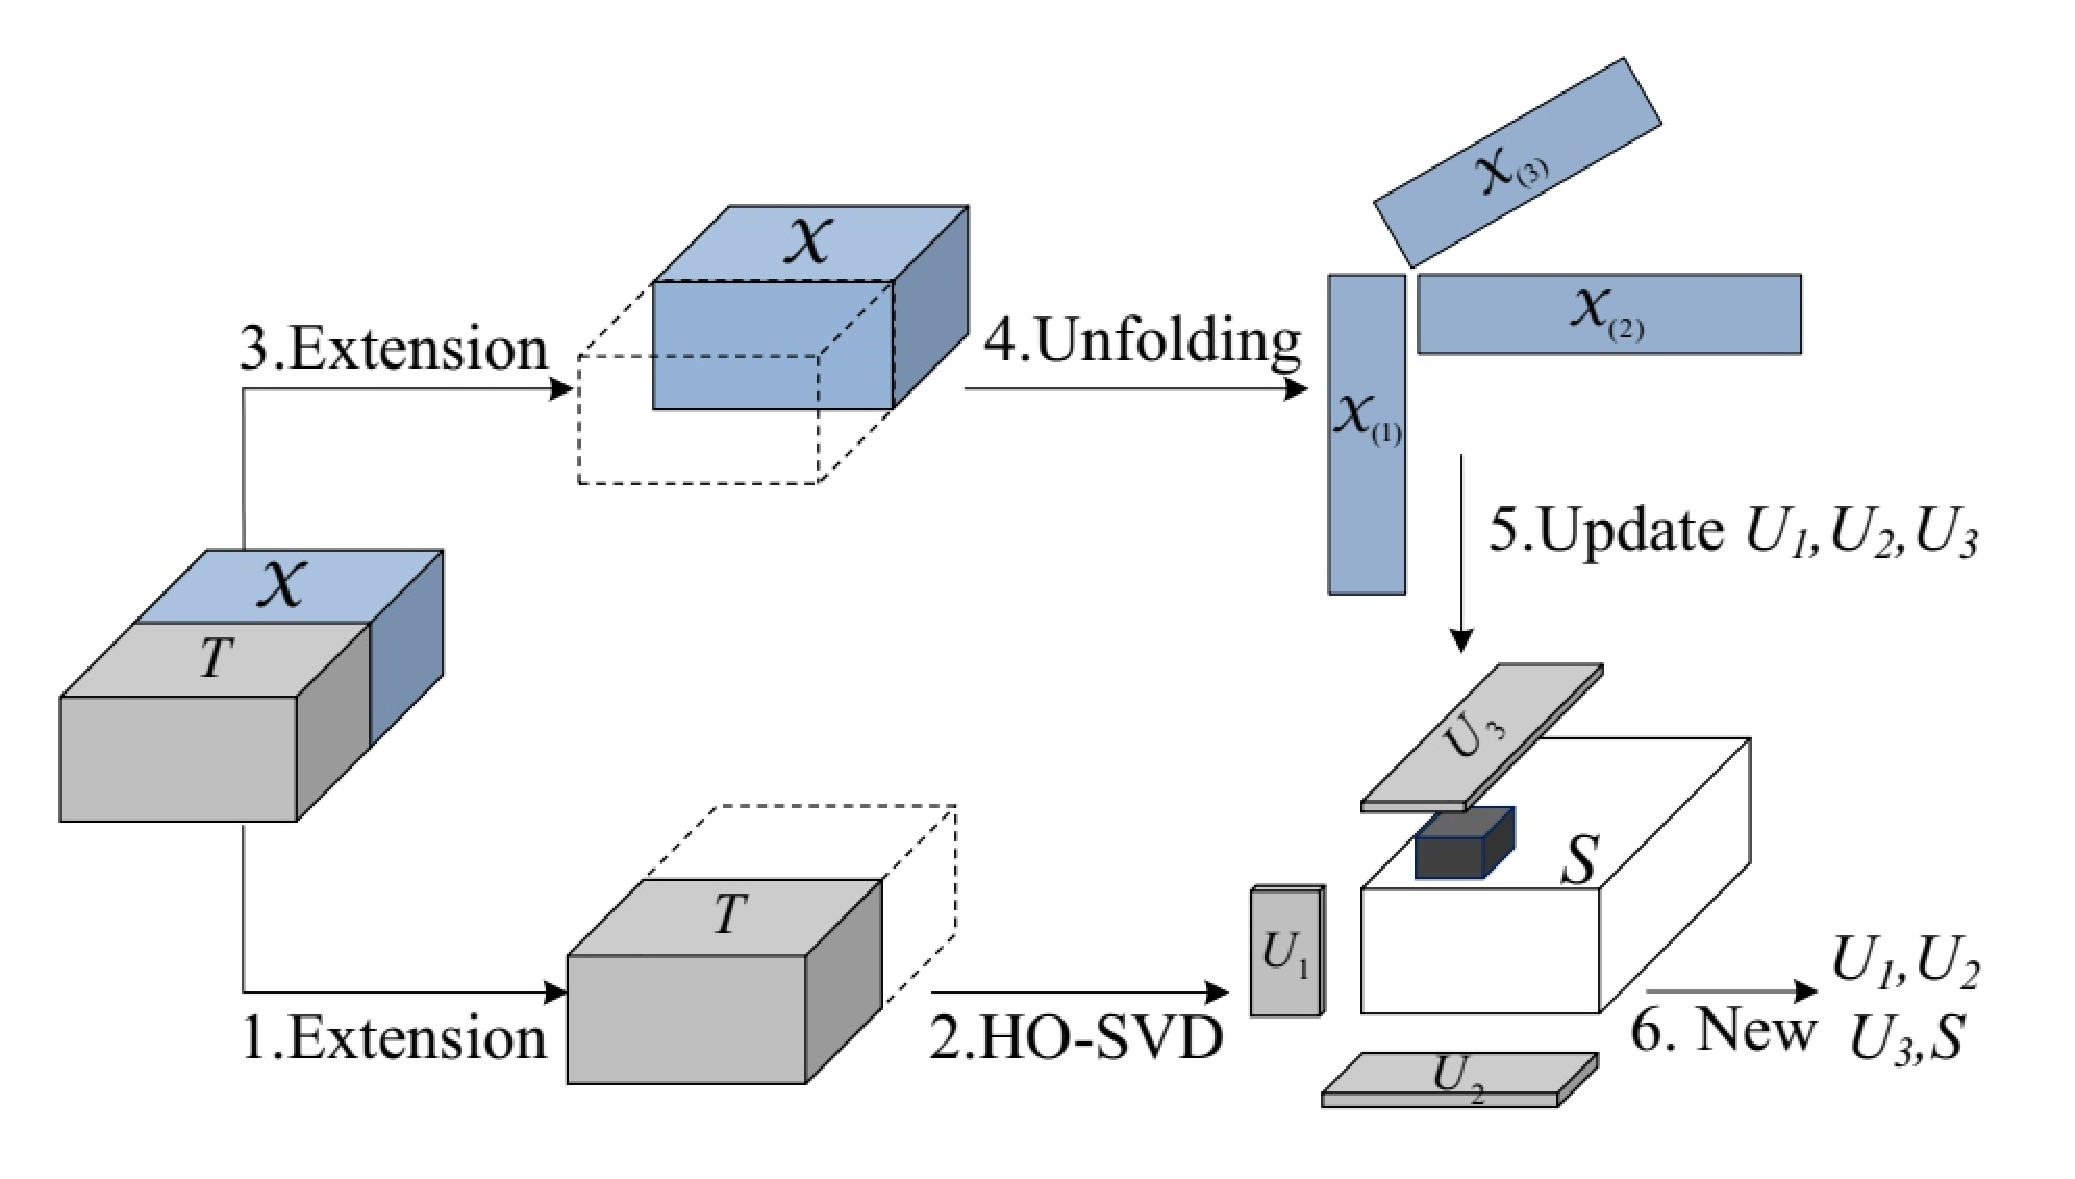
\includegraphics[width=.8\textwidth]{img/ok/AIHOSVD3.pdf}
\end{center}
\end{frame}
\begin{frame}
\begin{center}
	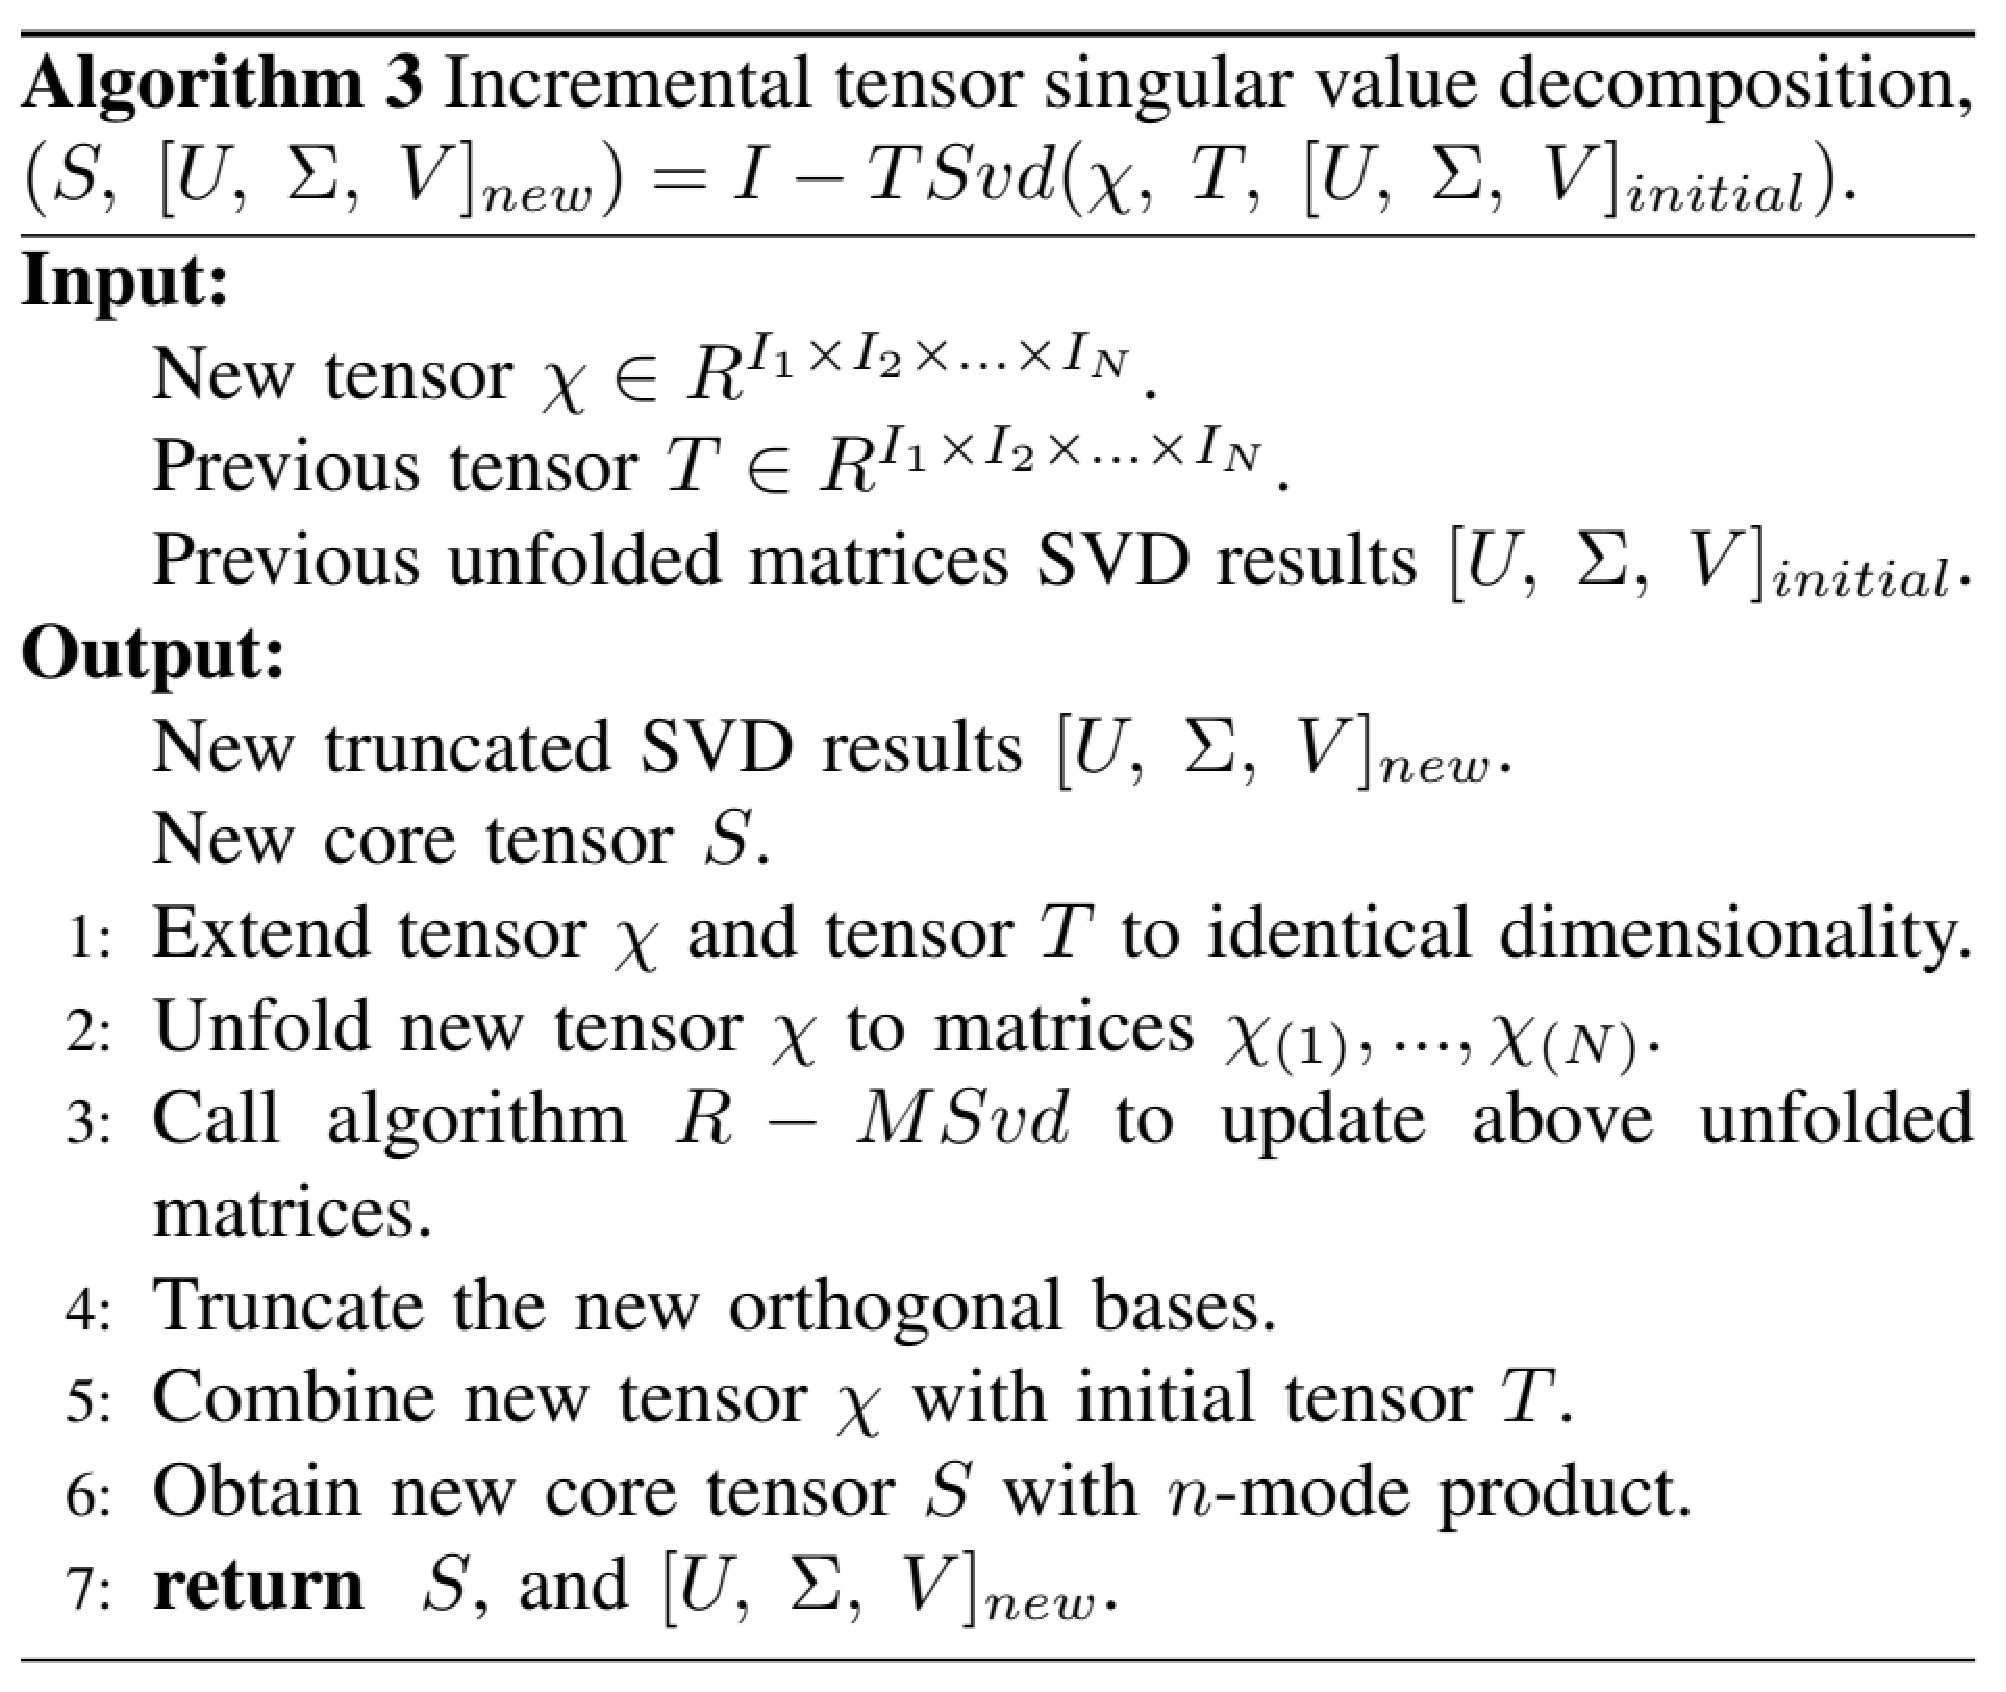
\includegraphics[width=.8\textwidth]{img/ok/AIHOSVD4.pdf}
\end{center}
\end{frame}
\begin{frame}{زمان پیچیدگی}
\small{
زمان محاسبه برای روش ارائه شده به صورت مجموع سه الگوریتم است که به صورت زیر محاسبه می‌شود:
\[Time=Time_{unf}+Time_{isvd}+Time_{prod}.\]
که عمله تبدیل unfolding  یک عمل از مرتبه 
$\mathcal{O}(1)$
است. زمان $Time_{isvd}$ مجموع زمان‌های مصرفی برای unfold کردن ماتریس $T_{(i)}$ است.
\begin{align*}
Time_N&=\sum_{i=1}^N Time_i\\
Time(n)&=\begin{cases}
C_1,&n=1\\
Time(n-1)+C_2,&n>1
\end{cases}
\end{align*}
پس زمان کل برابر $\mathcal{O}(k^2n)$ است.

}
\end{frame}